% Mitchell Hopkins's cover letter
% Last revision 6th Oct 23

% document setup
\documentclass{article}

% set font to default sans-serif
\usepackage[OT1]{fontenc}
\renewcommand*\familydefault{\sfdefault}

% packages to be used
\usepackage{graphicx}
\usepackage{fancyhdr}
\usepackage[margin=1.25in]{geometry}
\usepackage[dvipsnames]{xcolor}
\usepackage{hyperref}
    \hypersetup{colorlinks=true,linkcolor=RoyalBlue,urlcolor=RoyalBlue}
\usepackage{blindtext}

% remove paragraph indent
\setlength{\parindent}{0pt}

\begin{document}

% header and footer
\pagestyle{fancy}
\fancyhf{}
\title{Curriculum Vitae}
\author{Mitchell Hopkins}
\setlength\headheight{43pt}
\fancyhead[CO,CO]{\color{darkgray}\bfseries\Large{{Mitchell Hopkins}} \\ \small{\href{mailto:mh@artydh.io}{mh@artydh.io} | \href{https://linkedin.com/in/artydh}{https://www.linkedin.com/in/artydh} | {+}44 77633 51192}}
\fancyfoot[CO]{\color{gray}\small\emph{References available upon request.}}

\hspace*{0.5\linewidth}

% company address
\begin{minipage}{0.4\linewidth}
Company \par
Address 1 \par
Address 2 \par
City \par
Country / Postcode \par
\today
\end{minipage} \bigskip

To whom it may concern, \par \bigskip

\blindtext\medskip
\blindtext\medskip
\blindtext\medskip
\blindtext\medskip

Sincerely, \par \medskip

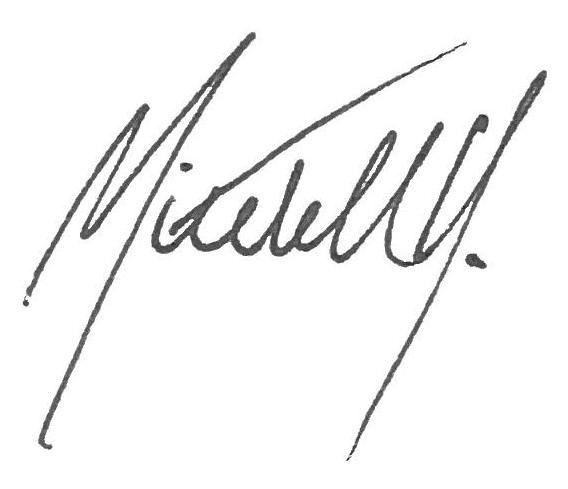
\includegraphics[height=4\baselineskip]{sig}\par
Mitchell Hopkins \par
\end{document}